\section{声波测距}
\subsection{实现}
本次大作业的声波测距部分基于 beepbeep 算法,具体实现在 \fileref{distance} 文件夹下。该文件夹下分别有测距的发送方,\fileref{distance/sender.py}、测距的接收方 \fileref{distance/receiver.py}、以及基于PyAudio库的录音模块 \fileref{distance/recorder.py}。 
\subsubsection{发送方}
对于发送方,首先使用tcp连接与接收方进行通信。发送方向接收方发送发送方准备就绪的信息,待收到接收方的准备就绪信息后,发送持续 0.5 秒,频率从 4000Hz 到 6000Hz 的线性调频信号。与此同时进行录音。

对于录音得到的结果,首先使用带通滤波器过滤掉噪音。然后将获得的信号与线性调频信号时序取反过后的信号进行卷积,根据卷积公式,卷积最大的那个点就是信号的起始位置$p_{A_1}$。

同样地,再接收到接收方的持续0.5秒,频率从 6000Hz 到 8000Hz 的线性调频信号。相应地通过卷积计算出信号的起始位置$p_{A_2}$。

则发送方接受到的信号时间差为以下公式,其中fs代表采样率。
$$
\Delta t_A = t_{A_1} - t_{A_2}=\frac{p_{A_1}-p_{A_2}}{fs}
$$
在发送方接收到接收到接收方传回来的起始位置之差$p_{B_1}-p_{B_2}$后,同样计算出时间差:
$$
\Delta t_B = t_{B_1} - t_{B_2}=\frac{p_{B_1}-p_{B_2}}{fs}
$$
计算出时间差后,由 beepbeep 算法:计算出两个电脑之间的距离:
$$
D = \frac{c}{2}(\Delta t_A - \Delta t_B) + d_{AA} + d_{BB}
$$
其中$d_{AA} , d_{BB}$分别代表两台电脑之间扬声器与麦克风之间的距离,$c$为声速,本次实验中取$340m/s$
\subsubsection{接收方}
对于接收方,在收到放松方发来的准备就绪信号后向发送方传回接收方准备就绪的信号,同时开始录音,在开始录音过后的1.5s后,发送接收方的线性调频信号。

与发送方类似地,接收方计算出接收方收到发送方信号的起始点$p_{B_1}$与接收方信号的起始点$p_{B_2}$,并将两个起始点之差通过 TCP 连接发送给发送方。

\newpage

\subsection{测试}
本次实验由于是基于传播时间的,时间差偏离 0.0058s 测距结果就会偏离 1s,因此,本次实验对环境及其敏感,其与麦克风、扬声器的质量,信号音量大小等因素息息相关,因此,下述测量结果仅代表本机测量结果。

\subsubsection{距离对性能的影响}

\iffalse
\begin{table}[h!]
    \centering
    \begin{tabular}{ccc}\toprule
        距离(cm)& 测量误差均值(cm) & 测量误差方差 \\\midrule
        \bottomrule
        50  & 6.89 & 4.88 \\
        100  & 9.54 & 6.32 \\
        150  & 22.31 & 12.47 \\
        200  & 38.32 & 8.23 \\ 
    \end{tabular}
\end{table}
\fi

\begin{figure}[h!]
    \centering
    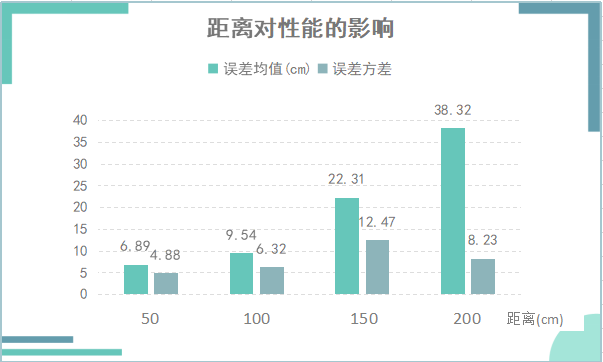
\includegraphics[width=0.6\linewidth]{1.png}
\end{figure}

\subsubsection{环境噪声的影响}

测量距离为100cm

\iffalse
\begin{table}[h!]
    \centering
    \begin{tabular}{ccc}\toprule
        环境& 测量均值(cm) & 测量方差 \\\midrule
        \bottomrule
        安静  & 109.54 & 6.32 \\
        人声说话  & 111.32 & 5.92 \\
        嘈杂音乐  & 163.50 & 25.68 \\
    \end{tabular}
\end{table}
\fi

\begin{figure}[h!]
    \centering
    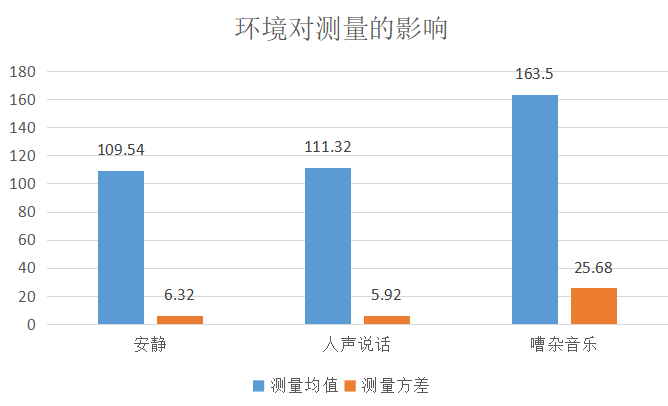
\includegraphics[width=0.6\linewidth]{2.png}
\end{figure}

\newpage

\subsection{遮挡物对性能的影响}

测量距离为100cm

\iffalse
\begin{table}[h!]
    \centering
    \begin{tabular}{ccc}\toprule
        遮挡物& 测量均值(cm) & 测量方差 \\\midrule
        \bottomrule
        无  & 109.54 & 6.32 \\
        人体  & 183.20 & 33.72 \\
        书籍  & 112.32 & 12.38 \\
    \end{tabular}
\end{table}
\fi

\begin{figure}[h!]
    \centering
    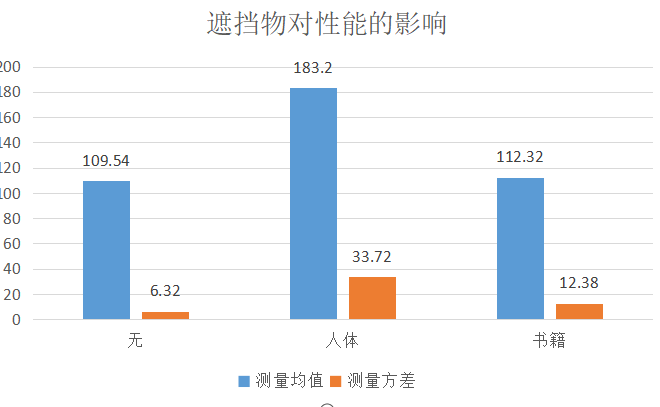
\includegraphics[width=0.6\linewidth]{3.png}
\end{figure}